\subsubsection{\gah}

In order to combine the benefits of \gads speed  and \gaana accuracy in the local search, we introduce \gah combining both approaches.

The exhaustive search over the local neighbors significantly impacts overall exploration performance. It evaluates many alternatives ($ \sum_{1 .. \lvert P \rvert} Steps_{i} * N * (\lvert T \rvert - N)$). Even considering only 1 step for each chromosome ($\lvert T \rvert$ = 50, $N$=10), already 5600 alternatives are evaluated. Hence, the fastest evaluation possible is paramount. To achieve this, \gah employs a two step approach: it first uses the faster (but less accurate) DS to identify a group of best neighbor candidates, and then re-evaluates those using the more accurate (but slower) Analytical Model to find the best neighbor. See \figref{fig:GAHybrid}. 

\gah first uses the faster evaluation \emph{DS} to find through exhaustive search the $N$ best neighbors ($Ch_{BN0}$ .. $Ch_{BNN}$) for a given chromosome $Ch_{cur}$. It then uses the analytic evaluation to select the best neighbor $Ch_{BN}$ from these candidates. The termination and random chromosome insertion are identical to \gads.

Dimensioning the group size is a local speed/accuracy trade-off. For our experiments, we opt to compare the top 5 neighbor candidates. We postulate that DS is sufficiently accurate to delineate from 400 down to 5 candidates ($\lvert T \rvert$ = 50, $N$=10). In addition, finding the absolute best in each step is not necessary as the search is iterative, improving in the next local step (or generation).


%\begin{figure}[htbp]
%	\centering
%	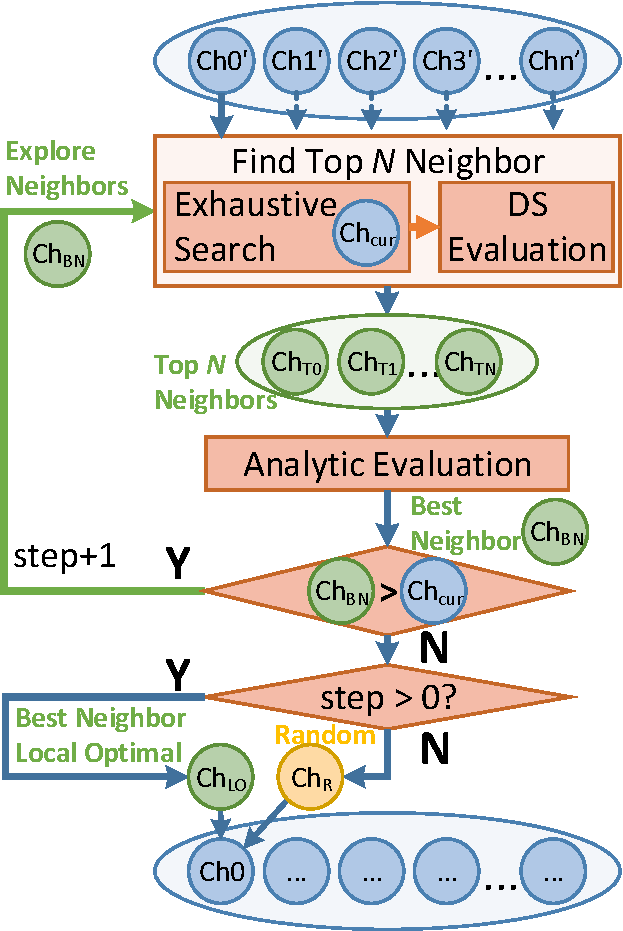
\includegraphics[width=0.48\linewidth]{fig/pGADSSA.pdf}
%	\caption{Guided Local Search (Hybrid)}
%	\label{fig:GAHybrid}
%\end{figure}